\gls{igro} is a web based \gls{gui} for the analysis and the integration of multiple \gls{ngs} data with the aid of several already published packages designed for this aim. 

For the \gls{gui} implementation we used the R \textit{Shiny} libraries because of its power to render R code in web format.

The tool presents itself with a main upper menu of main topics organized by scope. For each of this topic, a sub-menu with specific functionalities is available.
Moreover, depending on the selected functionality, a side menu is presented with additional functionalities or with input parameters to setup the specific tool.
After the parameter setup the results in graphical or table format are presented in the main part of the interface. (figure \ref{fig:integrhomain})

Before to proceed to its data analysis, it is mandatory for the user to setup the project with a dedicated interface. 
The user has to upload a design matrix which describes the information related to its samples, some of them are mandatory as the filename (with path) of the BAM files and the condition of each sample, while others are optional as the tissue or the run id. It is also possible to edit the design matrix by hand directly from the interface.
In such a way \gls{igro} creates in the working directory (returned by the \lstinline!getwd()! function) a dedicated folder with all the required subfolders and stores all the basic information of the project into an ad-hoc designed \lstinline!R6ProjectClass! which will be re-used during the whole session to speed up the configuration of each step of the analysis.

\begin{figure}[H]
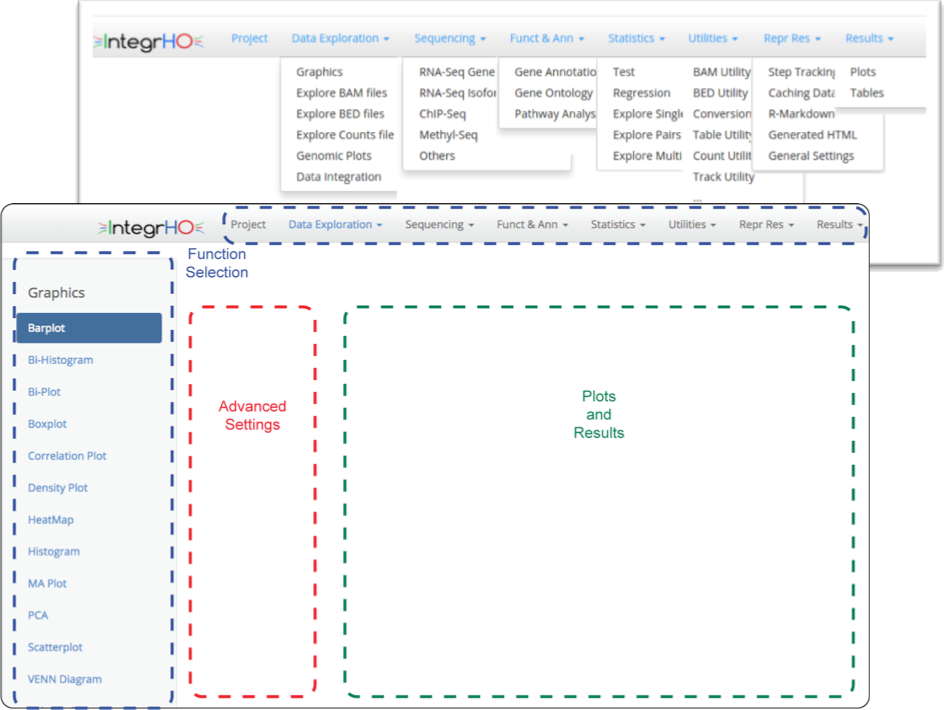
\includegraphics[width=\textwidth, keepaspectratio]{img/integrho/general_description.png}
\caption[integrho main interface]{}
\label{fig:integrhomain}
\centering
\end{figure}
 
\gls{igro} implements several functionalities and methodologies for \textit{RNA-Seq}, \textit{ChIP-Seq} and \textit{ATAC-Seq} data analysis, complementing these aspects by providing methodologies for their integration at different levels, as functional enrichment with Gene Ontology and Pathways,  peaks and genes annotation, and more statistical methods, as mixOmics, working with high-dimensional datasets.

For each -omics, \gls{igro} takes as input the BAM files, previously defined in the design matrix of the main project definition interface.

For each step of the analysis of each -omics, we tried to select more than one method to perform that task. 
In so doing we give the possibility to try different approaches in order to compare the final results, tuning the methods on the basis of the dataset under investigation.

For \textit{RNA-Seq} we constructed a dedicated interface for each step of a standard RNA-Seq data analysis pipeline, such as to build a count matrix, to filter out low counts with multiple tests, to normalize them and to account for batch effect. 
Moreover, we selected multiple methods for \gls{deg}, such as \textit{edgeR}, \textit{DESeq2}, \textit{NOISeq}.

For \textit{ChIP-Seq} we constructed specific interfaces for peak calling, annotation and \glspl{der} detection.
For the peak calling, because of the lack of specific methods starting from BAM files, we implemented interfaces for the DEScan2 and the \textit{csaw}\cite{Lun2015} peak callers. The first one born for broad peaks identification and the second one for both broad and narrow peaks quantification.
For the annotation we chose the \textit{ChIPpeakAnno} and the \textit{ChIPseeker} R/Bioconductor, which produces similar output formats starting from peaks. While for the detection of \glspl{der} we used the same methods as for \textit{RNA-Seq}.

For \textit{ATAC-Seq} we used mostly the same methods implemented for the \textit{ChIP-Seq}, but designing specific interfaces for the filtering/alignment and the counting matrix as implemented in the DEScan2 package (see chapter \ref{sec:descan2cap} for further details).

To provide an integration of these -omics, we dedicated an entire section to this aspect, with functionalities for the annotation of \glspl{der} with \glspl{deg} using \textit{ChIPpeakAnno} and to use this information to investigate the functional response by enriching for Gene Ontology or for Pathways.
These last two aspects implemented with aid of \textit{g:Profiler} \cite{Reimand2016} and \textit{graphite} \cite{Sales2012a} R/Bioconductor packages.

Moreover, to work with high-dimentional data sets, we are working on the implementation of methods like mixOmics, which gives a graphical response of the samples or the features, using two different methods diablo and mint.